\begin{figure*}
    \centering
    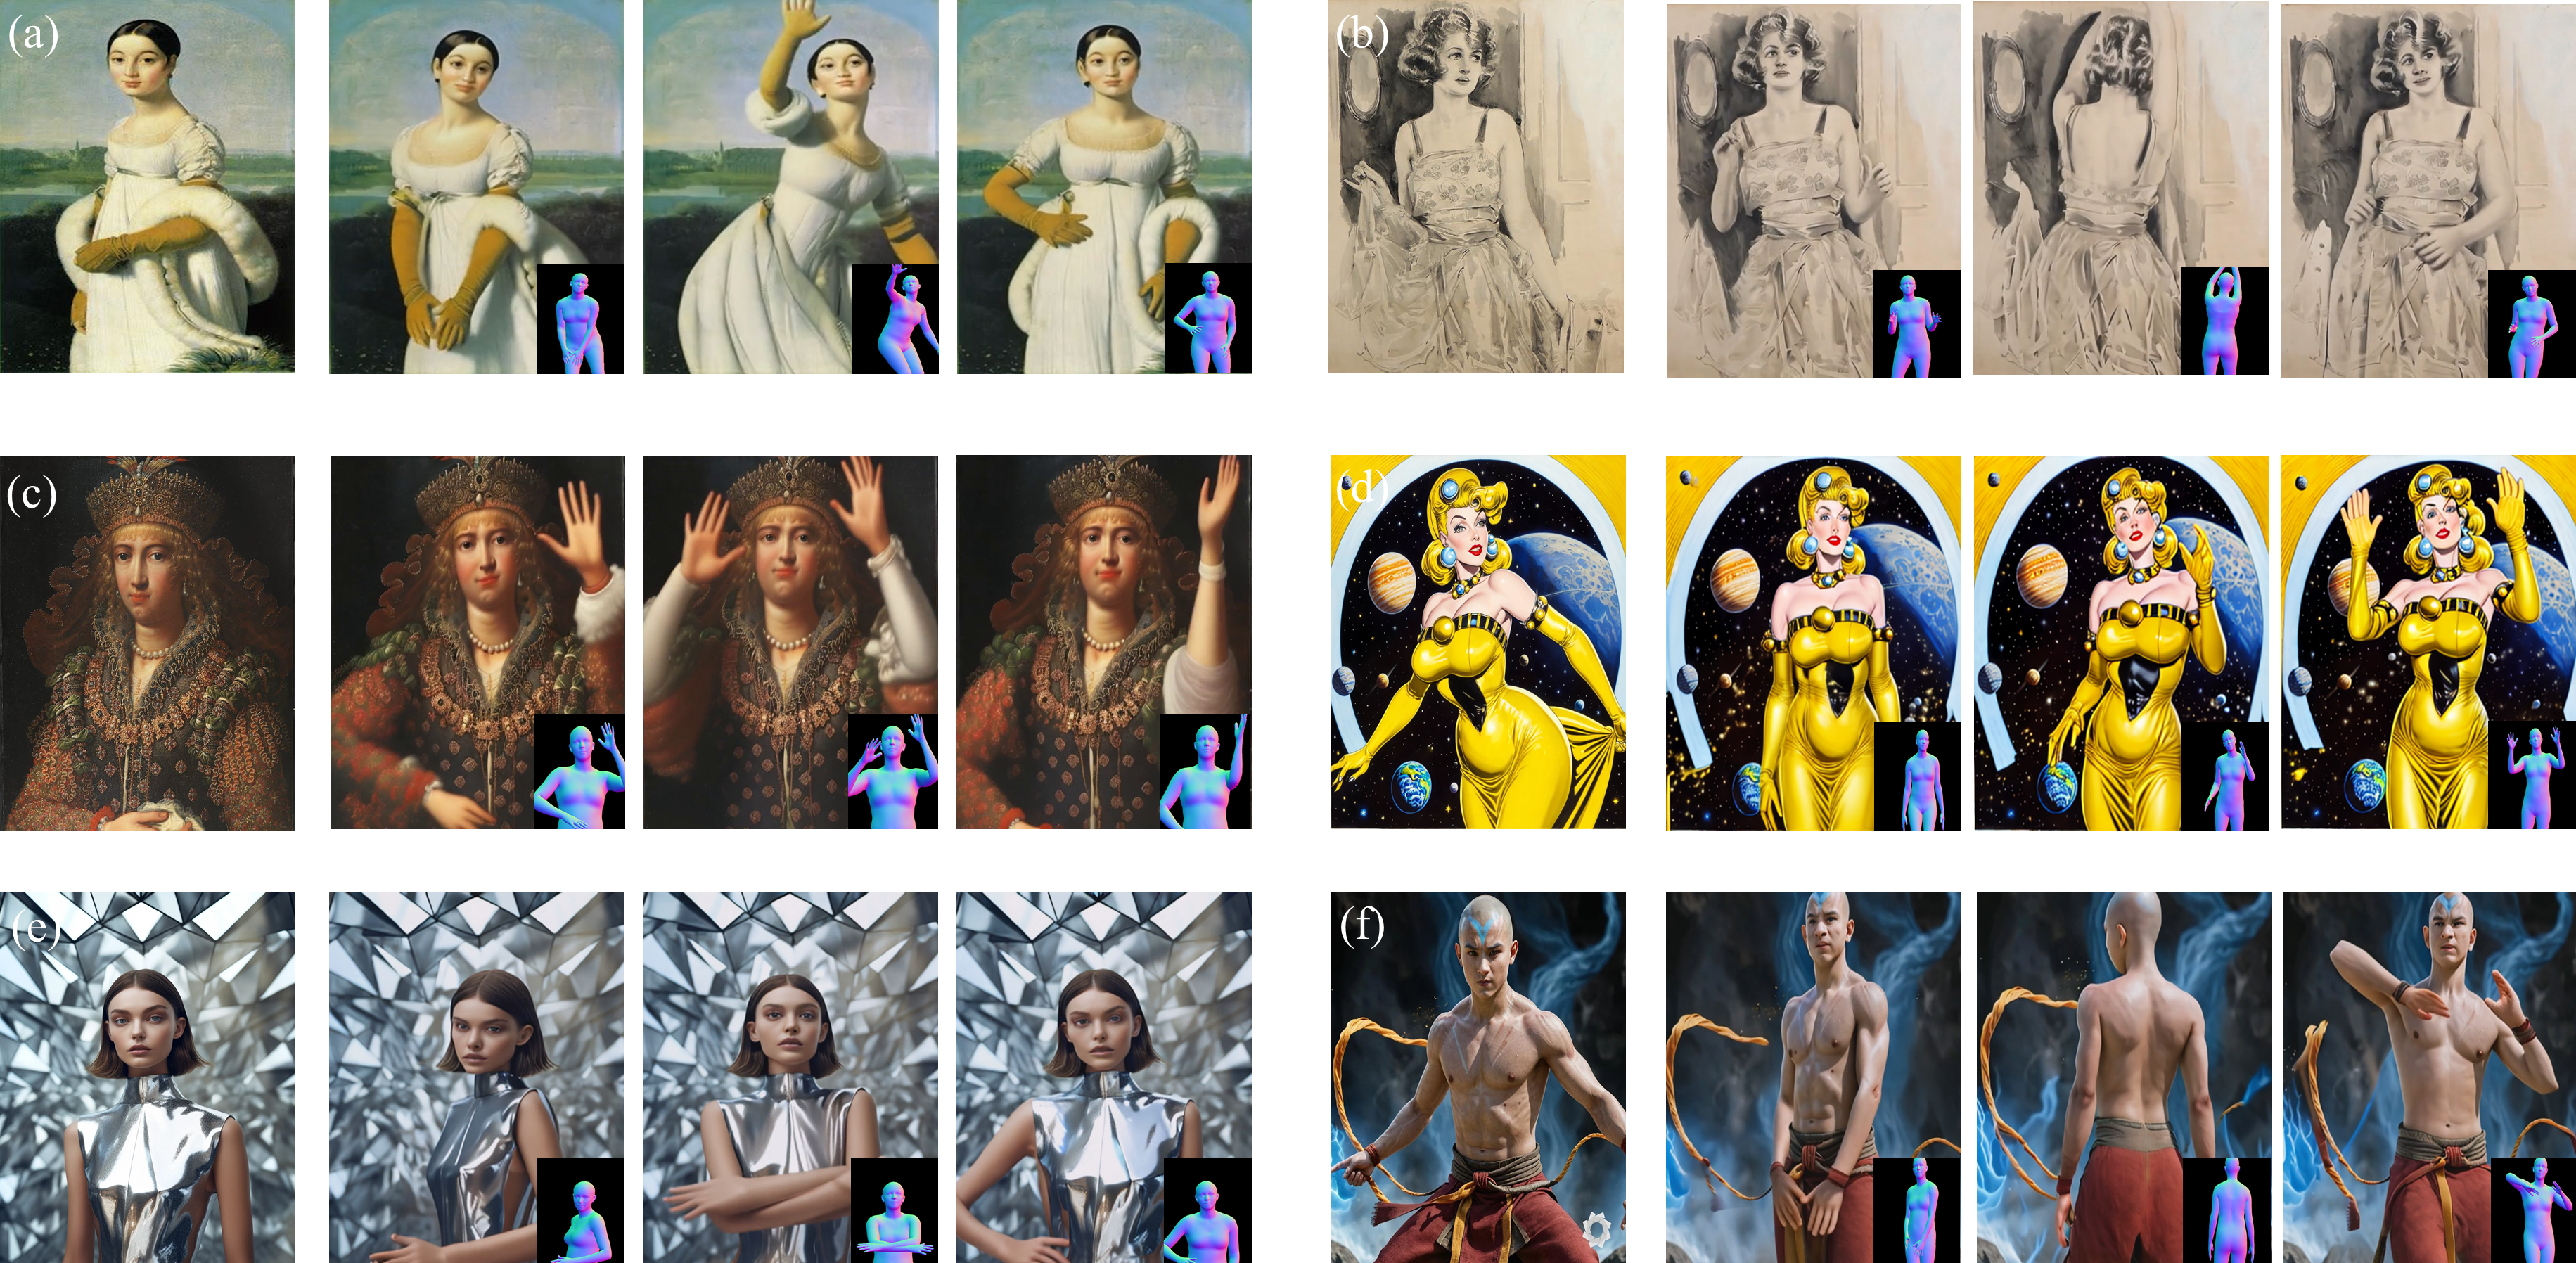
\includegraphics[width=1\linewidth]{figs/teaser.jpg}
    \caption{Demonstration of the proposed approach. Given a reference image, an audio sequence, and a textual prompt, the method generates animated portraits from frontal or different perspectives while preserving the portrait identity over extended durations. Additionally, it incorporates dynamic foreground and background elements, with temporal consistency and high visual fidelity. }
    \label{fig:enter-label}
    \vspace{-5mm}
\end{figure*}

\section{Introduction}
Portrait image animation refers to the process of generating realistic facial expressions, lip movements, and head poses based on portrait images. 
This technique leverages various motion signals, including audio, textual prompts, facial keypoints, and dense motion flow. 
As a cross-disciplinary research task within the realms of computer vision and computer graphics, this area has garnered increasing attention from both academic and industrial communities. 
Furthermore, portrait image animation has critical applications across several sectors, including film and animation production, game development, social media content creation, and online education and training.

In recent years, the field of portrait image animation has witnessed rapid advancements. 
Early methodologies predominantly employed facial landmarks—key points~\cite{siarohin2019first,zakharov2020fast,zhang2022sadtalker} on the face utilized for the localization and representation of critical regions such as the mouth, eyes, eyebrows, nose, and jawline. 
Additionally, these methods~\cite{gao2023high,ren2021pirenderer,zhang2023metaportrait,champ2024} incorporated 3D parametric models, notably the 3D Morphable Model (3DMM)~\cite{blanz2003face}, which captures variability in human faces through a statistical shape model integrated with a texture model. 
However, the application of explicit approaches grounded in intermediate facial representations is constrained by the accuracy of expression and head pose reconstruction, as well as the richness and precision of the resultant expressions.
Simultaneously, significant advancements in Generative Adversarial Networks (GANs) and diffusion models have notably benefited portrait image animation. 
These advancements~\cite{corona2024vlogger,liu2024anitalker,tian2024emo,wei2024aniportrait,xu2024vasa,zhang2024tora,champ2024} enhance the high-resolution and high-quality generation of realistic facial details, facilitate generalized character animation, and enable long-term identity preservation. 
Recent contributions to the field—including Live Portrait~\cite{guo2024liveportrait}, which leverages GAN technology for portrait animation with stitching and retargeting control, as well as various end-to-end methods such as VASA-1~\cite{xu2024vasa}, EMO~\cite{tian2024emo}, and Hallo~\cite{xu2024hallo,cui2024hallo2} employing diffusion models—exemplify these advancements.

Despite these improvements, existing methodologies encounter substantial limitations. 
First, many current facial animation techniques emphasize eye gaze, lip synchronization, and head posture while often depending on reference portrait images that present a frontal, centered view of the subject. 
This reliance presents challenges in handling profile, overhead, or low-angle perspectives for portrait animation. Secondly, accounting for significant accessories, such as holding a smartphone, microphone, or wearing closely fitted objects, presents challenges in generating realistic motion for the associated objects within video sequences.
Third, existing methods often assume static backgrounds, undermining their ability to generate authentic video effects in dynamic scenarios, such as those with campfires in the foreground or crowded street scenes in the background.

Recent advancements in diffusion transformer~(DiT)-based video generation models~\cite{yang2024cogvideox, polyak2024movie, bao2024vidu, liu2024sora} have addressed several challenges associated with traditional video generation techniques, including issues of realism, dynamic movement, and subject generalization. 
In this paper, we present the first application of a pretrained DiT-based video generative model to the task of portrait image animation.
The introduction of this new video backbone model renders previous U-Net-based methods for identity maintenance, audio conditioning, and video extrapolation impractical. 
We tackle these issues from three distinct perspectives.
(1)~\textbf{Identity preservation}: We employ a 3D VAE in conjunction with a stack of transformer layers as an identity reference network, enabling the embedding and injection of identity information into the denoising latent codes for self-attention. This facilitates accurate representation and long-term preservation of the facial subject's identity.
(2)~\textbf{Speech audio conditioning}: We achieve high alignment between speech audio—serving as motion control information—and facial expression dynamics during training, which allows for precise control during inference. We investigate the use of adaptive layer normalization and cross-attention strategies, effectively integrating audio embeddings through the latter.
(3)~\textbf{Video extrapolation}: Addressing the limitations of the DiT-based model in generating continuous videos, which is constrained to a maximum of several tens of frames, we propose a strategy for long-duration video extrapolation. 
This approach uses motion frames as conditional information, wherein the final frames of each generated video serve as inputs for subsequent clip generation.

We validate our approach using benchmark datasets, including HTDF and Celeb-V, demonstrating results comparable to previous methods that are constrained to limited datasets characterized by frontal, centered faces, static backgrounds, and defined expressions. 
Furthermore, our method successfully generates dynamic foregrounds and backgrounds, accommodating complex poses, such as profile views or interactions involving devices like smartphones and microphones, yielding realistic and smoothly animated motion, thereby addressing challenges that previous methodologies have struggled to resolve effectively. 